\documentclass[justified, nobib, twosided]{tufte-book}

% Includes
\usepackage{amsmath}
\usepackage{mathtools}
\usepackage{physics}
\usepackage{siunitx}
\usepackage{booktabs}

% Set up bibliography
\usepackage[style=authoryear]{biblatex}
\bibliography{resources}

\usepackage{graphicx}
\graphicspath{ {figures/} }

\title{ASTR~356 \\ Final Project}
\author{Jackson Petty}

%%%% Kevin Godny's code for title page and contents from https://groups.google.com/forum/#!topic/tufte-latex/ujdzrktC1BQ
\makeatletter
\renewcommand{\maketitlepage}{%
\begingroup%
\setlength{\parindent}{0pt}

{\fontsize{24}{24}\selectfont\textit{\@author}\par}

\vspace{1.75in}{\fontsize{36}{54}\selectfont\@title\par}

\vspace{0.5in}{\fontsize{14}{14}\selectfont\textsf{\smallcaps{\@date}}\par}

\vfill{\fontsize{14}{14}\selectfont\textit{\@publisher}\par}

\thispagestyle{empty}
\endgroup
}
\makeatother

\titlecontents{part}%
    [0pt]% distance from left margin
    {\addvspace{0.25\baselineskip}}% above (global formatting of entry)
    {\allcaps{Part~\thecontentslabel}\allcaps}% before w/ label (label = ``Part I'')
    {\allcaps{Part~\thecontentslabel}\allcaps}% before w/o label
    {}% filler and page (leaders and page num)
    [\vspace*{0.5\baselineskip}]% after

\titlecontents{chapter}%
    [4em]% distance from left margin
    {}% above (global formatting of entry)
    {\contentslabel{2em}\textit}% before w/ label (label = ``Chapter 1'')
    {\hspace{0em}\textit}% before w/o label
    {\qquad\thecontentspage}% filler and page (leaders and page num)
    [\vspace*{0.5\baselineskip}]% after
%%%% End additional code by Kevin Godby

\begin{document}
	\maketitle
	\chapter{Introduction}

The Sloan Digital Sky Survey has, since its inception in 2000, collected high-quality photometric observations of objects in our universe. The third data release from the SDSS contains information on over 500 thousand different astronomical objects, classified into Galaxies, Quasars, Stars, M Stars, Sky Spectra, and Unknown Objects. It covers over 3700 square degrees of spectroscopic area.

Our project will focus on the statistical analysis of quasar data. Quasars, or quasi-stellar objects, are of great importance to astronomy and astrophysics. They are highly luminous active galactic nuclei, among the brightest objects in the universe, and help astronomers to understand galaxy formation and evolution. Quasars are often so bright that they shine through other astronomical objects, like clouds of dust or gas, leaving tell-tale absorbtion lines in quasar's spectra. All quasars yet observed have redshifts of between 0.1 and 7 (approximately), corresponding to distances of several hundered million to several billion light years away. Due to their large distance from Earth, studying quasars provides insight into the early stages of the universe~[\cite{starchild}, \cite{skyserver}].

\section{Statistical Goals}
This project will explore three distinct statistical analyses of SDSS quasar data. Firstly, we wish to preform \emph{Principle Component Analysis} on the data to attempt to reduce the dimensionality to a more reasonable level while still preserving enough variation in the data in order to preform further investigations. Second, we will preform polynomial regression on the $r-i$ color vs $z$ redshift to seek a predictor for the former based on the latter, along with residual analysis to determine what degree polynomial best approximates our data. To preform the analysis, we will make frequent use of the \texttt{numpy}, \texttt{scikit-learn}, and \texttt{scipy}. To plot data, we will use \texttt{matplotlib} and \texttt{astropy}. Finally, we will preform hypothesis testing on the $r$ band data to test if the data's parent distribution is Gaussian. We'll use various statistical tests to check the normality of the data, and use histograms to visualize the population distributions.

\section{Data}
The SDSS data set which we will be using in this analysis includes observations of $46,420$ Quasi-Stellar Objects, or quasars. Originally presented in \cite{schneider2005}, data includes photometric observations in the following features:\footnote{All magnitudes are in an inverted logarithmic scale.} \\[1ex]

\begin{tabular}{@{}rp{8cm}@{}}
	\toprule
	\textbf{\texttt{Des}} & SDSS Designation \\
	\textbf{\texttt{RA}} & Right Ascension, $0^\circ \leq \text{\textbf{\texttt{RA}}} \leq 360^\circ$. \\
	\textbf{\texttt{Dec}} & Declination, $-90^\circ \leq \textbf{\texttt{Dec}} \leq +90^\circ$. \\
	\midrule
	\textbf{\texttt{z}} & Redshift  \\
	\midrule
	\textbf{\texttt{U}} & Ultraviolet band, with $\lambda_\text{eff} \approx \SI{365}{\nano\meter}$. \\
	$\sigma_\text{\textbf{\texttt{U}}}$ & Measurement error in the ultraviolet band. \\
	\textbf{\texttt{G}} & Green band, with $\lambda_\text{eff} \approx \SI{464}{\nano\meter}$. \\
	$\sigma_\text{\textbf{\texttt{G}}}$ & Measurement error in the green band. \\
	\textbf{\texttt{R}} & Red band, with $\lambda_\text{eff} \approx \SI{658}{\nano\meter}$. \\
	$\sigma_\text{\textbf{\texttt{R}}}$ & Measurement error in the red band. \\
	\textbf{\texttt{I}} & Near-infrared band, with $\lambda_\text{eff} \approx \SI{806}{\nano\meter}$. \\
	$\sigma_\text{\textbf{\texttt{I}}}$ & Measurement error in the \textbf{\texttt{I}} near-infrared band. \\
	\textbf{\texttt{Z}} & Infrared band, with $\lambda_\text{eff} \approx \SI{900}{\nano\meter}$. \\
	$\sigma_\text{\textbf{\texttt{Z}}}$ & Measurement error in the \textbf{\texttt{Z}} near-infrared band. \\
	\textbf{\texttt{J}} & Infrared band, with $\lambda_\text{eff} \approx \SI{1220}{\nano\meter}$. \\
	$\sigma_\text{\textbf{\texttt{J}}}$ & Measurement error in the \textbf{\texttt{J}} near-infrared band. \\
	\textbf{\texttt{H}} & Infrared band, with $\lambda_\text{eff} \approx \SI{1630}{\nano\meter}$. \\
	$\sigma_\text{\textbf{\texttt{H}}}$ & Measurement error in the \textbf{\texttt{H}} near-infrared band. \\
	\textbf{\texttt{K}} & Infrared band, with $\lambda_\text{eff} \approx \SI{2190}{\nano\meter}$. \\
	$\sigma_\text{\textbf{\texttt{K}}}$ & Measurement error in the \textbf{\texttt{K}} near-infrared band. \\
	\textbf{\texttt{Radio}} & Radio brightness \\
	\textbf{\texttt{X-ray}} & X-ray brightness \\
	\midrule
	\textbf{\texttt{M}} & Absolute magnitude in the \textbf{\texttt{I}} band. \\
	\bottomrule
\end{tabular}

	\chapter{Principle Component Analysis}

\section{Theory}
\emph{Principle Component Analysis} is a process by which a multivariate data set, containing observations in multiple features, can be reduced to a data set with a lower dimensionality, aiding in computational complexity and visualization\footnote{It's quite difficult to plot data in 17-dimensional space, for example, but quite easy to plot data in 2-dimensional space.}. PCA works by attempting to identify various new features which maximize the variance of the original data, and from which we could most easily reconstruct the original characteristics of our observations.

These new features (the \emph{principle components} in PCA) act as a new set of axes along which we can plot and analyze our data. These components are identified using eigenvalue/eigenvector decomposision.\footnote{Recall that an \emph{eigenvector} is a vector which is not rotated under a linear transformation, it is only scaled. The scale factor, denoted by $\lambda$, is called the \emph{eigenvalue} of that vector.} Specifically, we preform decompoisition on the covariance matrix $\Sigma$ of our data. Consider an imaginary data set which has $m$ observations (perhaps of different celestial objects) in $n$ different features (color, redshift, right ascension, declination, etc.). The covariance matrix of this data set will be an $n \times n$ square matrix, where the $(i,j)$ entry represents the covariance of the $i$\textsuperscript{th} and $j$\textsuperscript{th} features in our data. Importantly, it is useful to note that $\Sigma$ is a \emph{square symmetric} matrix, since the covariance of the $i$\textsuperscript{th} and $j$\textsuperscript{th} features equals the covariance of the $j$\textsuperscript{th} and $i$\textsuperscript{th} features; mathematically,
\[ \operatorname{Cov}(X_i,X_j) = \operatorname{Cov}(X_j,X_i) \implies \Sigma_{ij} = \Sigma_{ji}. \]
Since $\Sigma$ is square symmetric, we know it is diagonalizable\footnote{This is a direct consequence of the \emph{spectral theorem}.} into a new matrix whose entries are the eigenvalues of the principle components of the data set. Each eigenvalue represents the variance of the data along that new axis.
\[ \Sigma \sim \begin{pmatrix}
\lambda_1 & 0 & 0 & \cdots \\
0 & \lambda_2 & 0 & \cdots \\
0 & 0 & \lambda_3 & \cdots \\
\vdots & \vdots & \vdots & \ddots
\end{pmatrix} \]
By selecting the $k$ largest eigenvalues, we can reduce our original data set from $n$-dimensional space into $k$-dimensional space. The smaller our value of $k$, the simpler our model becomes, but we pay a price of explaining less and less of the underlying variance in the data. Our goal will be to strike a happy medium between the two, reducing our data to a visualizable range but preserving enough of the variation that we don't loose too much information.

\section{Application to SDSS Data}
As noted in the introduction, one of the greatest things about data from the Sloan Digital Sky Survey is that it has observations in many different features. The quasar data used in this project has 23 distinct values for each observation. Among these, one is a designation within the SDSS catalogue, and eight are error values for other observations. These values are not measured quantities, and don't really serve to explain observational features we might wish to use to analyze our data, so we won't include these in our original data set when preforming PCA.
\begin{marginfigure}
	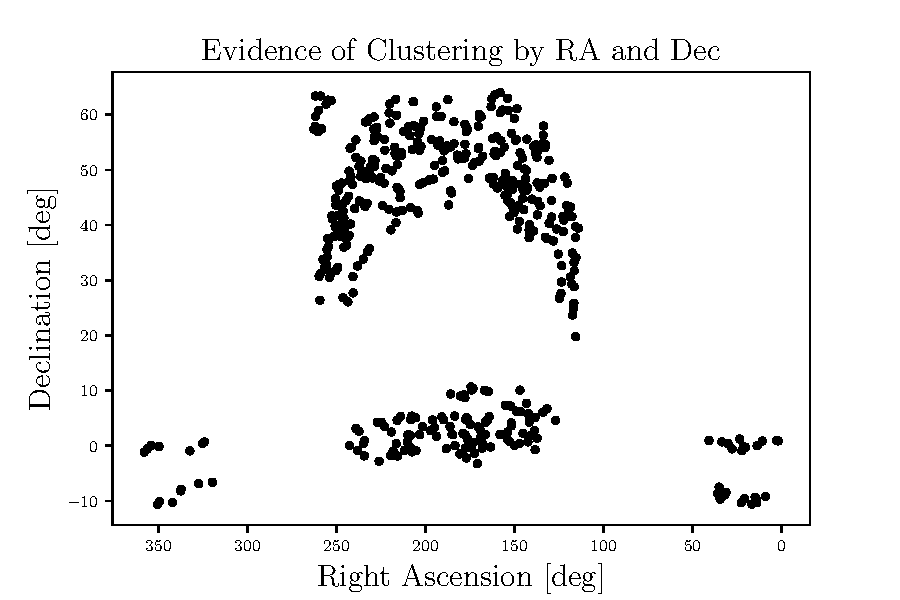
\includegraphics[width=2.3in]{ra-dec}
	\caption{Evidence of clustering in \texttt{RA} vs \texttt{Dec}. These clusters are apparent because the SDSS data only contains observations for certain regions of the sky, not because the data are demonstrative of quasar clusters in particular regions.}
	\label{fig:ra-dec}
\end{marginfigure}
\begin{marginfigure}
	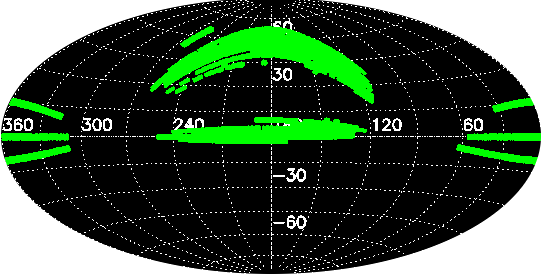
\includegraphics[width=2.3in]{dr3spectro_big}
	\caption{Map of spectral coverage from SDSS Data Release 3~[\cite{sdssWebsite}].}
	\label{fig:spec-cov}
\end{marginfigure}
Additionally, data in the \texttt{K\_mag}, \texttt{H\_mag}, and \texttt{J\_mag} features contain \texttt{NA} values when no value was observed for a particular quasar; if we included these three features in our analysis, PCA would find that the \texttt{NA} values would serve as an indicator for a group which doesn't exist, so these features are excluded from the analysis as well. Finally, we remove the Right Ascension and Declination values from the data, since the data form distinct observational clusters which arise from the limitations of the survey, and are not representative of actual clustering found in nature. Compare the \texttt{RA} vs \texttt{Dec} plot of quasar data in Figure~\ref{fig:ra-dec} to the map of spectral coverage from SDSS Data Release 3 in Figure~\ref{fig:spec-cov}. This leaves the data set with nine distinct features for analysis.

Observations of radio and X-ray brightness also contain some missing values; since these values come from compilations of different astronomical surveys (NRAO FIRST for radio data, ROAST All-Sky Survey for X-ray data), it only makes sense to include observations which have complete data in both categories. Thus, we must mask our original data to exclude partial observations, or else the \texttt{NA} values present will again serve as indicator variables for clusters which don't exist. Fully reducing our data set, we are left with $456$ observations in $9$ features.

We conduct Principle Component Analysis on the data using \texttt{scikit-learn}'s \texttt{PCA} tool. The first task is to find the optimum number of components to which we should reduce our data. Such a value is found by comparing the explained variance in the reduced data set by the number of components in that data set. In general, we expect that increasing the number of components will explain more of the variance in the data, but increasing the number of components too much will result in data that cannot be easily visualized.
% or worked with in a meaningfully more efficient way than working with the unreduced data would entail.

\begin{figure}
	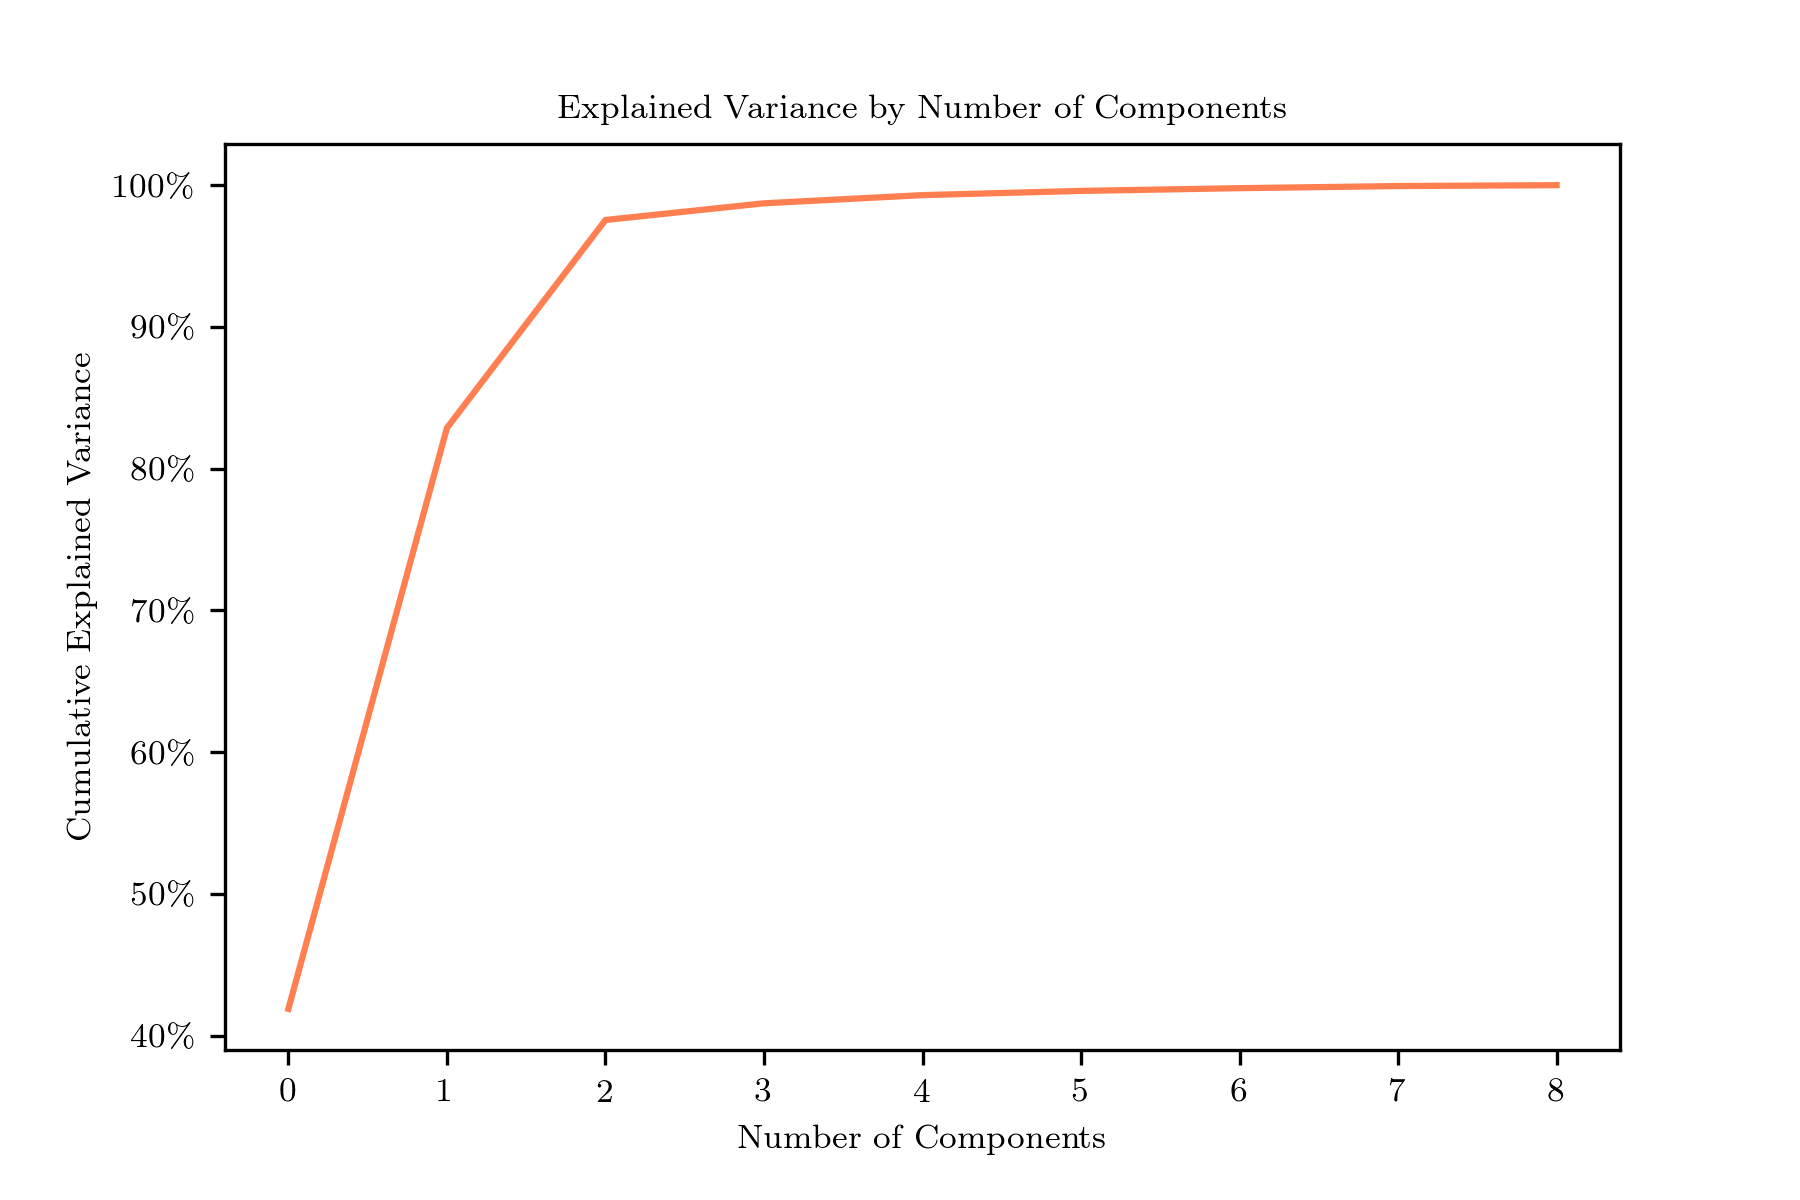
\includegraphics[width=\textwidth]{exp-var}
	\caption{As we increase the number of components in our reduced data set, the explained variance increases. Notice that after $n=2$, each additional component contributes minimally to the cumulative explained variance.}
	\label{fig:exp-var}
\end{figure}

As shown in Figure~\ref{fig:exp-var}, we find that the first two principle components explain over $97.5\%$ of the total variance in our data set, indicating that we can safely reduce the dimensonality of the quasar data to just two components. For ach additional component ($n = 3, \dots, 8$), we see diminishing returns to how much we can explain the variance in our data. Adding a third principle component gets us to $98.7\%$ of the total variance, and a fourth pushes us to over $99\%$ of the total variance, but we loose the ability to adequately visualize the data.

\begin{figure}
	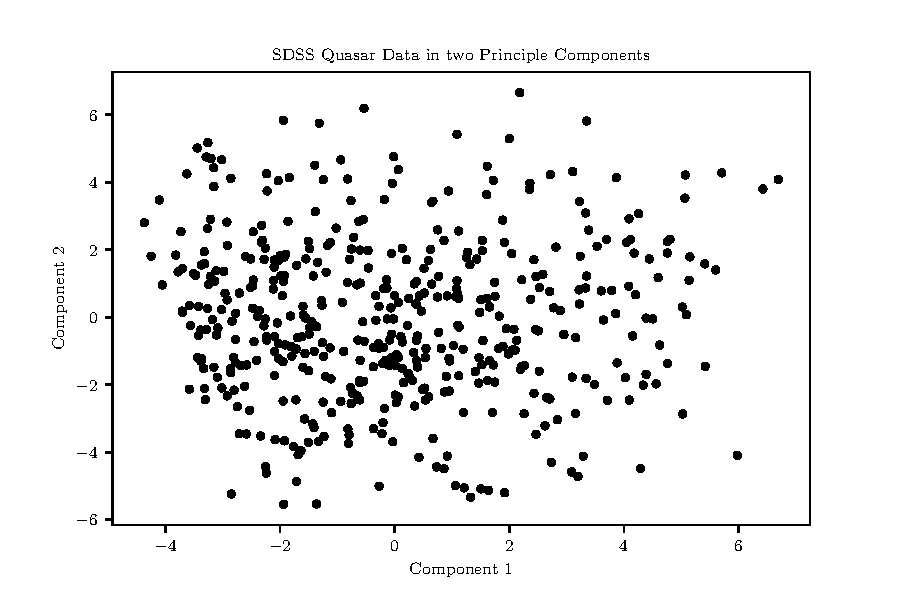
\includegraphics[width=\textwidth]{pca-reduced}
	\caption{Our original 456 observations in 9-dimensional data projected into a two-dimensional visualization.}
	\label{fig:pca-red}
\end{figure} 
While Figure~\ref{fig:pca-red} shows it is now much easier to graph our data, we do lose about $2.5\%$ of the total explained variance using this lower-dimensional model. We also lose the ability to physically understand exactly \emph{what} each axis represents. While before, we could have plotted the data in color-radio magnitude space, we now only have `Component 1' and `Component 2', which represent some linear combination of the original features.
	\chapter{Regression}

\section{Statistical Theory}
Regression is the process by which we estimate the relationships among variables by fitting values to a line or curve in order to predict one value based on another. In its simplest form, regression is a linear estimate of a single variable in terms of another. In this case, we have a set of observations in one variable $Y$ and in another variable $X$, and we see a linear relationship 
\[ y_i = \beta x_i + m \]
which allows us to predict the value of $Y$ given a value of $X$. Nature, however, is never so keen, and we always deal with errors in our measurements of $X$ and $Y$, which means that it is nigh impossible to find an \emph{exact} relationship between two variables. Instead, we seek to find the \emph{best} relationship we can, where the goodness of a particular linear model is determined by the \emph{residuals}, or errors between our predicted values and our actual measurements. In this case, an estimate $\hat{y}_i$ replaces our actual measured value $y_i$ in the above equation.

The easiest way of analyzing how well a given model fits the data is to look at the squared sum of the residuals,
\[ \text{SSQ} = \sum (\hat{y}_i - y_i)^2. \]
Model's which fit a particular data set well will have a lower squared sum of residuals, while a model which fits poorly will have a higher value. Ideally, we want this statistic to trend to zero, but it is often impossible to get arbitrarily low values for SSQ due to the presence of random noise in our data and the limits in precission of our measurement tools. Another closely related measure of how good our model fits is the $\chi^2$ statistic, defined as 
\[ \chi^2 = \sum \frac{(\hat{y}_i - y_i)^2}{\sigma_i^2}. \]
This introduces a new term, $\sigma_i^2$, the variance in our measurement. This weights the SSQ by how confident we are in a given residual; if we are very confident of a value, and our expected value differs from our measured value, then it is a bigger deal that if we are uncertain in the measurement to begin with.

However, it isn't always that case that the relationship between two variables is linear. It may be quadratic, cubic, logarithmic, exponential, sinusoidal, or any number of other types of relation. In these cases, we determine the complexity of the fit by the number of free parameters we must estimate. For the case of our simplistic linear regression from above, we must estimate \emph{two} parameters: $m$ and $\beta$. In general, a polynomial regression of degree $d$ will have $d + 1$ free parameters, given by the coefficients of the polynomial and the intercept. While this is a more reasonable estimate of how wrong our model is, it is still succeptable to the problem of \emph{over-fitting}. Namely, we can always reduce the errors in our fits by introducing more complexity in our model, but this obscures the actual relationship between the two variables we want to analyze. For example, if we had 200 data points, we could fit a 200-degree polynomial and end up with a $\chi^2$ statistic of zero; however, this likely isn't a good model to explain the relationship between our two variables.

To solve this, we introduce penalties for having \emph{too many parameters} in our model. The Reduced $\chi^2$ statistic divides through by the degrees of freedom, equal to number of observations $n$ minus the number of free parameters $m$.
\[ \chi^2_\nu = \frac{\chi^2}{\nu} = \frac{\chi^2}{n - m} = \frac{\chi^2}{n - (d + 1)}. \]

\section{Aplication to SDSS Data}
Unlike principle component analysis, the SDSS quasar data contains observations for all color bands as well as as for redshift, meaning that we do not need to preform any subsetting of our data; instead, we can preform a polynomial regression on all 46,000 observations included in the original data set. Our goal will be to find a predictor for color based on the redshift of a quasar. We'll separate color out by band and preform an inital plot of color versus redshift to get a sense of general trends in the data, as shown in Figure~\ref{fig:color-redshift}.

\begin{figure}
	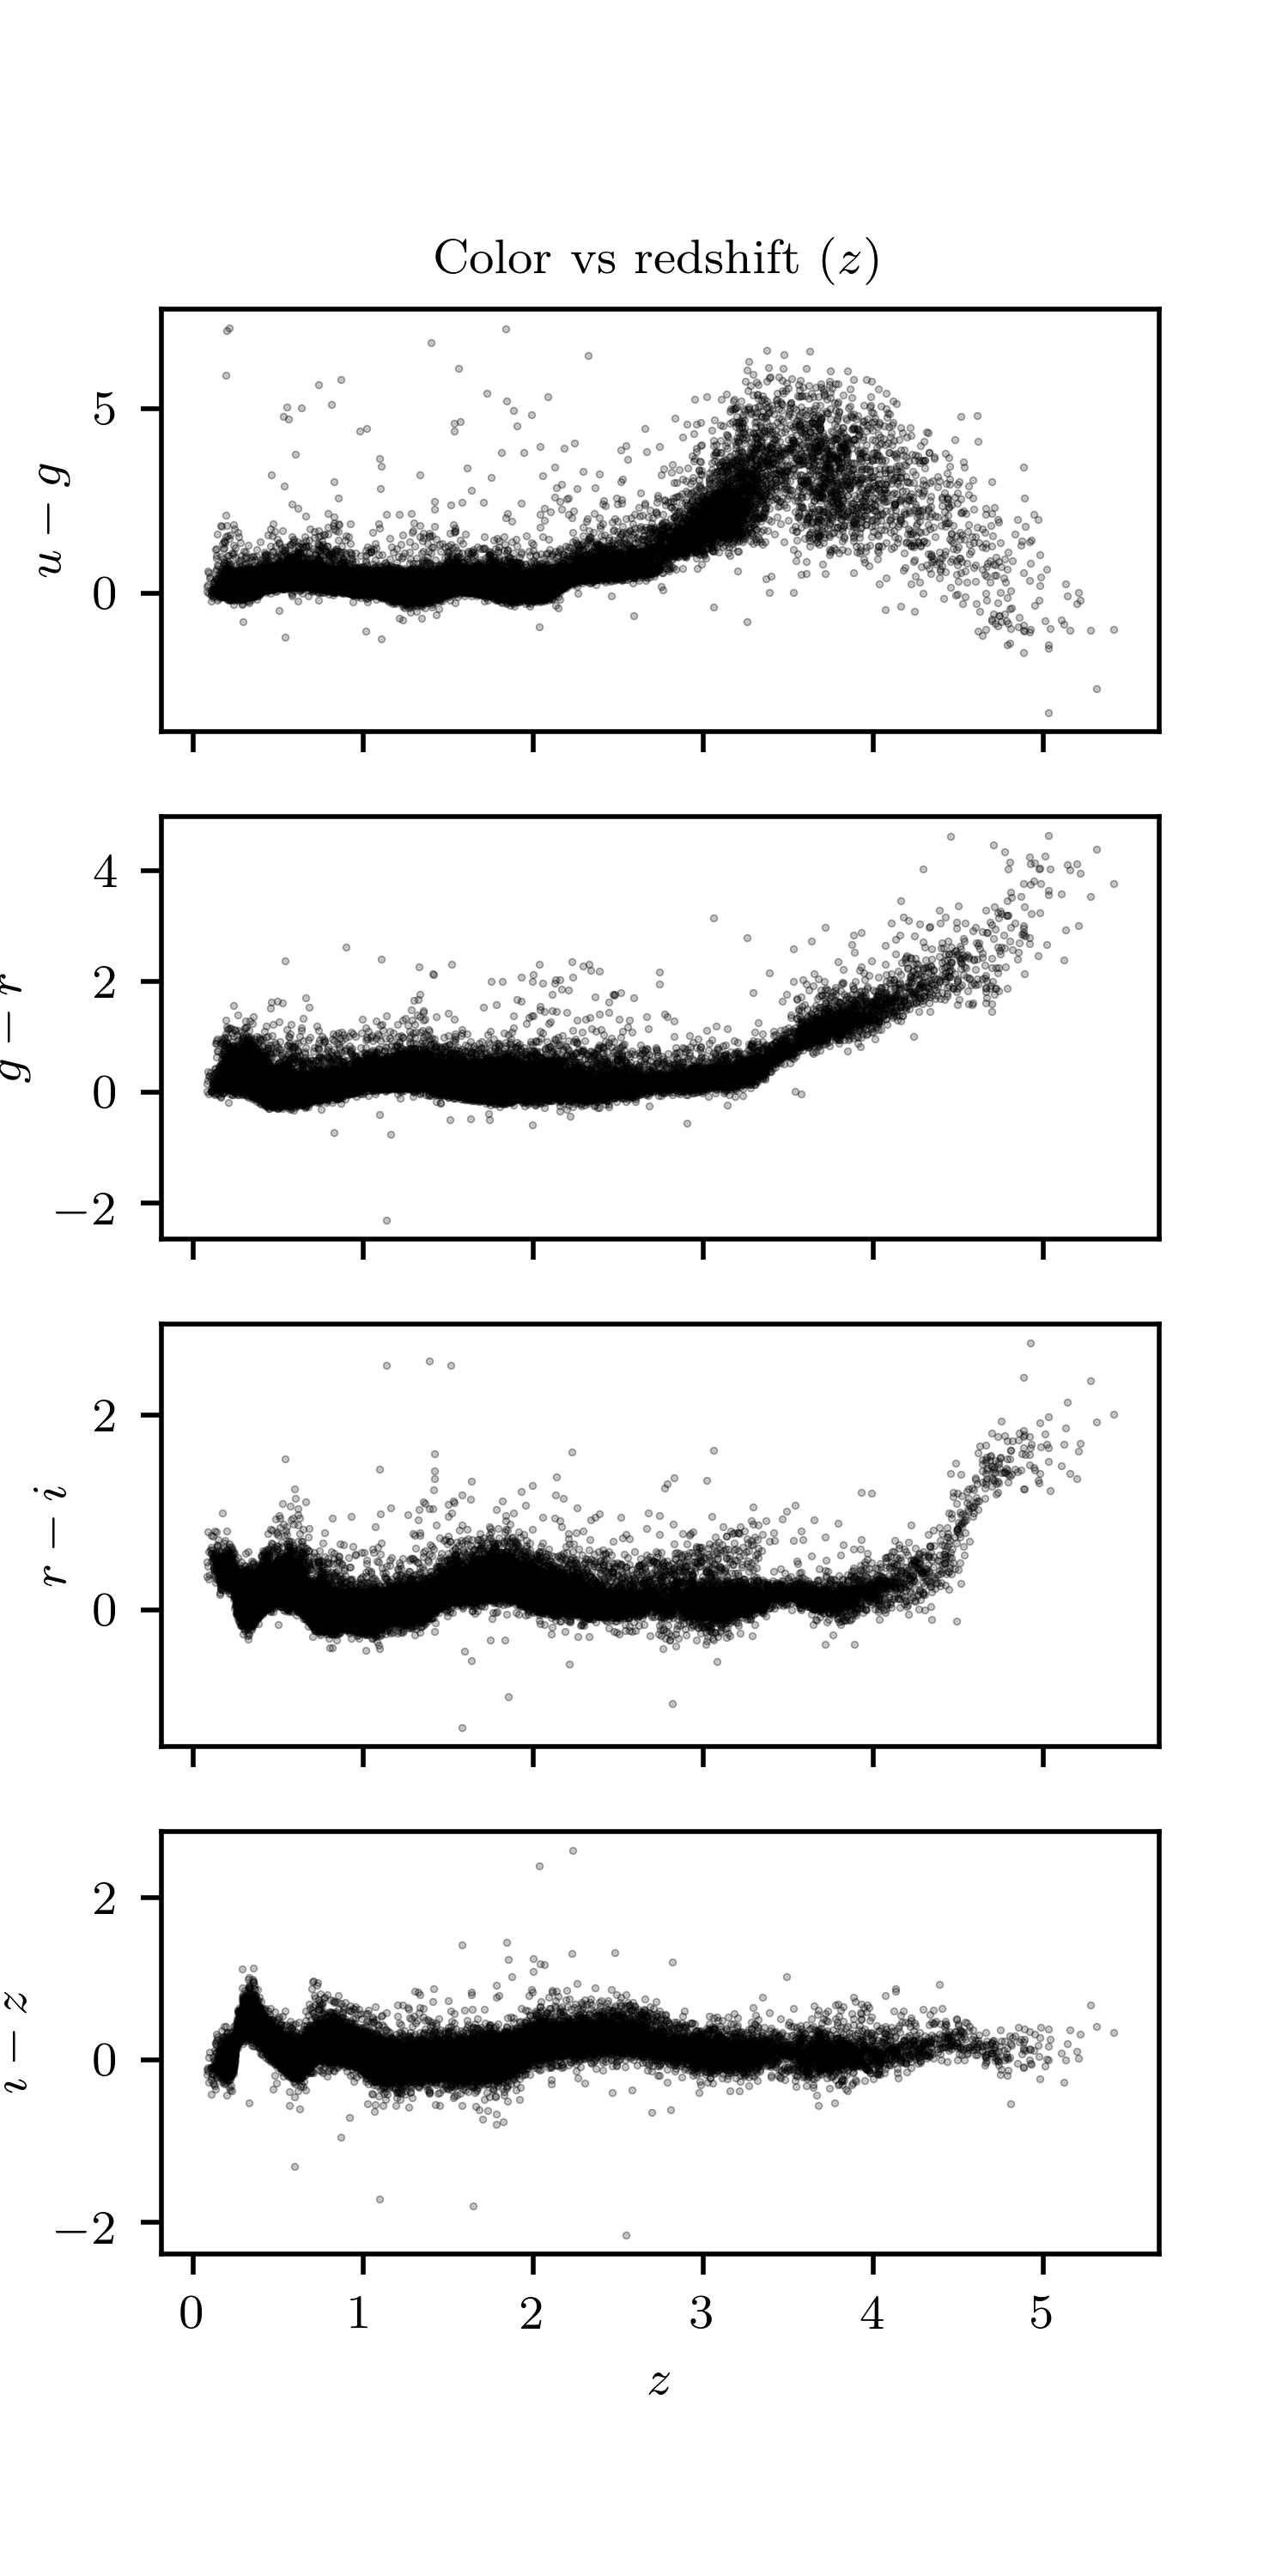
\includegraphics[width=\textwidth]{color-redshift}
	\caption{Color vs redshift plots for four different color bands ($u-g$, $g-r$, $r-i$, and $i-z$). For the sake of brevity, we will only find a regression for one of these relations, namely $r-i$ vs $z$.}
	\label{fig:color-redshift}
\end{figure}

We fit polynomials of degree $0$ through $15$ to our data, and find the $\chi^2$, Adjusted $R^2$, Akaike and Bayesian Information Criterions for each. Figure~\ref{fig:reg-err} shows these values by degree. For $\chi^2$, AIC, and BIC, lower is better, while we want a high adjusted $R^2$ value.
\begin{figure}
	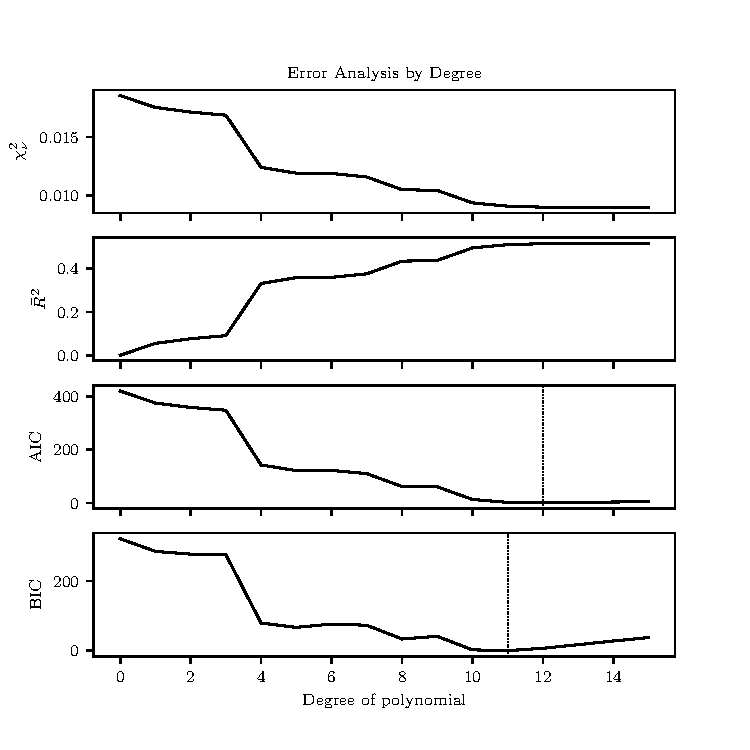
\includegraphics[width=\textwidth]{reg-err}
	\caption{Residual analysis and information criterion plots for polynomial regressions of degree $d$. The vertical lines at $d = 12$ and $d = 11$ represent the degrees which minimize the Akaike and Bayesian Information Criterion's respectively, indicating the polynomials which best fit the data without overfitting the data.}
	\label{fig:reg-err}
\end{figure}

We can also use cross validation to test how well polynomials of a certain degree predict the data when fitted to only a subset of it. We preform cross validation by randomly splitting our $r - i$ band measurements into a training set and cross validation set, and fitting a polynomial to the training data, and then calculating the $\chi^2$ value for the training and cross-validation data separately.
\begin{figure}
	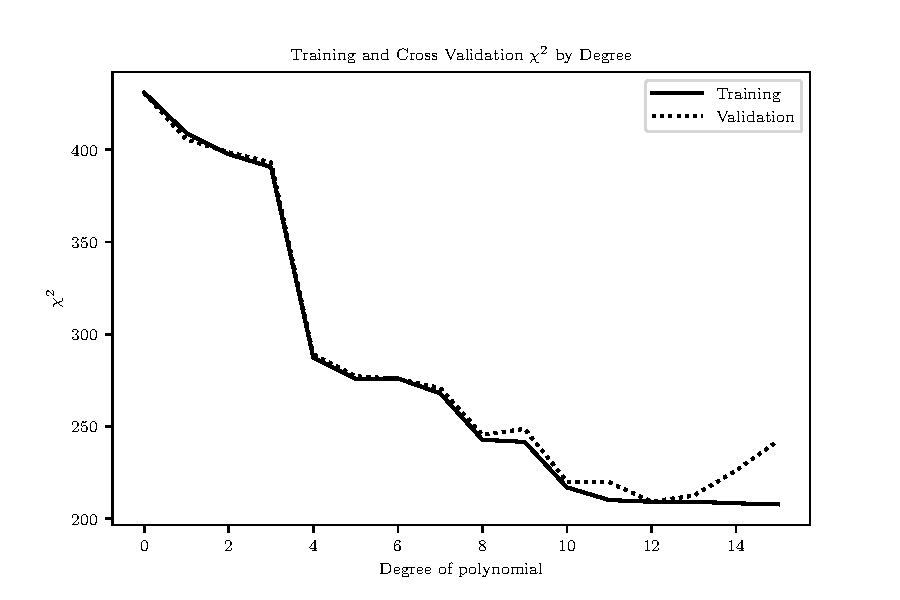
\includegraphics[width=\textwidth]{cross-val}
	\caption{Cross validation of polynomial fit by degree. Notice that for $d > 13$, the $\chi^2$ value begins to start increasing, indicating that past this point our regressions no longer adequately serve as predictors for the cross validation subset.}
	\label{fig:cross-val}
\end{figure}
Notice in Figure~\ref{fig:cross-val} that $\chi^2$ is minimized for the training data for all $d \geq 11$, while $\chi^2$ is minimized for the testing data for $d = 12,13$. After this point, we see a noticible uptick in the $\chi^2$ value, indicating that for degrees greater than $12$, the polynomial regressions no longer predict random subsamplings of our data better. This tells us that a degree of $11$, $12$ or $13$ is best suited to our data. To visualize our optimal regressions, we plot the polynomials of best fit, overlaying the data points in Figure~\ref{fig:best-reg}.

\begin{figure}
	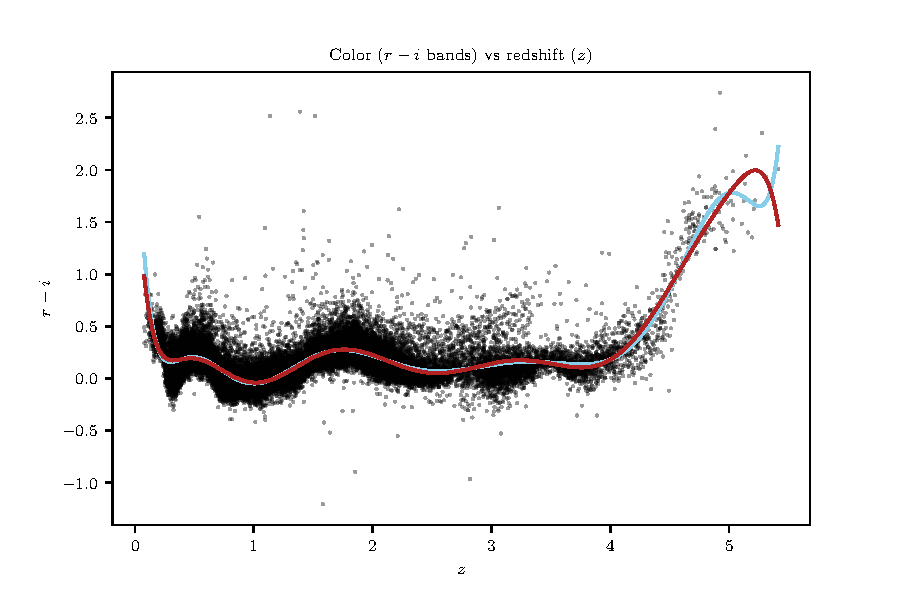
\includegraphics[width=\textwidth]{ri-redshift-deg}
	\caption{Polynomial regressions of degree $11$ (red) and $12$ (blue) for $r - i$ vs $z$. These polynomials are those which minimize the AIC and BIC.}
	\label{fig:best-reg}
\end{figure}
Both the $11$ and $12$ degree polynomials are similar to the results found by~\citeauthor{wu2003} in 2004, although the exact polynomials are not listed in their paper.

	\chapter{Hypothesis Testing \& Normality}

\section{Statistical Theory}
When preforming statistical analysis, we often want to check whether or not our assumtions about data are justified. This is the realm of \emph{hypothesis testing}, where we formulate testable hypothesis about whether our data fits a given model, and then preform various statistical tests on that data to support or reject our hypothesis.

The crux of all hypothesis testing comes in the creation of two mutually exclusive outcomes for our tests. These are the \emph{null hypothesis} and the \emph{alternative hypothesis}. The null hypothesis, often written $H_0$, is a hypothesis which is ``created to be rejected'' in favor of the alternative hypothesis, $H_a$. The most common example of hypothesis testing comes in the testing of normality of our data. Here, we want to establish whether or not a normal Gaussian distribution is a reasonable parent distribution for our data. In many cases, this is a reasonable initial guess for the distribution of data, but (unsurprisingly) not all data comes from Gaussian distributions. When testing for normality, we often formulate our hypothesis as follows:
\begin{itemize}
	\item $H_0$ is the hypothesis that our data is drawn from a normal distribution.
	\item $H_a$ is the alternative, that the data was \emph{not} drawn from a normal distribution.
\end{itemize}

To provide a quantitative way to evaluate these hypothesis, we turn to the actual statistical tests. In general, statistical tests require an \emph{a priori} selection of a confidence level, denoted $\alpha$. This is a measure of ``how strict do we want our test to be?'' Lower values of $\alpha$ mean that our tests need to be ``more sure'' of their results to reject or fail to reject the null hypothesis. Closely related to the confidence level is the $p$-value; this is a measure of ``how sure our test actually is'' of our result, loosely speaking. In general, we are able to reject the null hypothesis when $p < \alpha$; this is why picking a smaller $\alpha$ makes it harder to reject $H_0$.

There are two main tests we can use to test for normality: the \emph{Shapiro-Wilk} test and the \emph{Anderson-Darling} test~[\cite{nist}]. The Shapiro-Wilk test gives a statistic\footnotetext{For the Shapiro-Wilk test, $x_{(i)}$ are the ordered sample values (in ascending magnitude), and $a_i$ are constants generated from a normal distribution with $n$ samples and the same mean and variance of the sample data.} \[ W = \frac{\qty(\sum_{i=1}^n a_ix_{(i)})^2}{\sum_{i=1}^n (x_i - \bar{x})^2}, \]
along with an associated $p$-value. The Anderson-Darling test calcualtes the statistic $A^2$, along with critical values $v_\text{crit}$ for various confidence levels. Given an $\alpha$, we choose the critical value for that confidence level and compare it to $A^2$; if $A^2 > v_\text{crit}$, we reject $H_0$, otherwise we fail to do so.

It is important to note that rejecting or failing to reject the null hypothesis are not conclusive tests for normality, or a lack thereof. Failing to reject the null hypothesis \emph{does not} imply that the alternative hypothesis is true, it merely points suggestively in that direction while winking. We also must contend with the fact that for extremely large sample sizes (on the order of tens of thousands of data points), these tests become increasingly sensitive to even minor fluctuations in the data. This can lower the validity of these test in relation to our data, so we often look for other ways to analyze the normality of data. One such method is a normal quantile plot, which divides the sample data into quantiles and plots them according to what would be expected if the data were drawn from a Gaussian. If the data is indeed normal, the quantile plot looks roughly linear.

\section{Application to SDSS Data}
\subsection*{Examining Normality with Histograms}
We'll begin by examining a histogram of $r$ band magnitude observations of quasars in the full SDSS data set.
\begin{figure}
	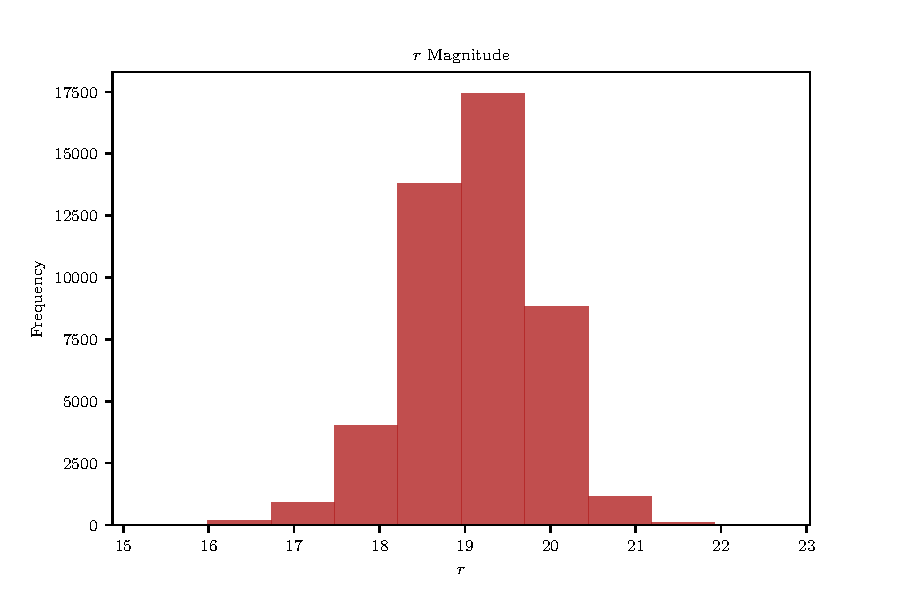
\includegraphics[width=\textwidth]{hist}
	\caption{Histogram of $r$ band magnitudes. The bin width is the default from \texttt{matplotlib}'s \texttt{hist()} function. Changing the bin width may reveal a more complicated distribution than appears in this histogram.}
\end{figure}
As we can clearly see from the graph, the $r$ band magnitude peaks somewhere between 19 and 20, and tapers off quickly to either side. From a distance, these data \emph{do} appear to be normally distributed, but the only way to get a quantitative estimate of the data's normality is to preform additional statistical tests on it. 

\subsection*{Statistical Tests for Normality}
Given that our data looks normal from a distance, we can use various tests to, well, test the normality of our data. First, we must formulate a hypothesis to test. We'll say that the null hypothesis $H_0$ is the hypothesis that our data is drawn from a Gaussian distribution. We choose an $\alpha$ of $0.01$.

First, we'll preform the Shapiro-Wilks test, to obtain a test statistic $W$ and associated $p$-value. If our $p$-value is \emph{less} than the chosen $\alpha$, we have evidence that our data is not drawn from a normal parent distribution, and we can reject $H_0$. Using \texttt{scipy.stats.shapiro()}, we obtain the following values:
\[ W \approx 0.99,\quad p \approx 0.0. \]
Since $p < \alpha$, we reject the null hypothesis under the Shapiro-Wilks test, and conclude that our data is \emph{not} normally distributed.

Next, we'll use the Anderson-Darling test to investigate normality. From this, we will obtain the test statistic $A^2$ and an associated critical value which we'll compare to investigate if the data is normally distributed. Using \texttt{scipy.stats.anderson()}, we obtain the following values:
\[ A^2 \approx 129.4, \quad v_\text{crit} = \begin{pmatrix}
	0.576 \\ 0.656 \\ 0.787 \\ 0.918 \\ 1.092
\end{pmatrix}, \]
where the critical values are for significance levels of $15\%$, $10\%$, $5\%$, $2.5\%$, and $1\%$ respectively. Since we are using $\alpha = 0.01 = 1\%$, we select the largest critical value, $v_\text{crit} = 1.092$. To analyze the results, we must compare $A^2$ to $v_\text{crit}$. Since
\[ A^2 \gg 1.092, \]
we reject $H_0$ and again conclude that our data is not normally distributed.

It is important to note that both the Shapiro-Wilks and Anderson-Darling tests suffer from the issue that for large sample sizes, the tests may detect departures from normality that are not really present in the data. Since our sample size is large (over $46,000$ data points), these results may not be conclusive in discovering departures from normality. To further investigate this, we will use a \emph{Q-Q} plot to plot theoretical quantiles against the quantiles observed in our data.
\begin{figure}
	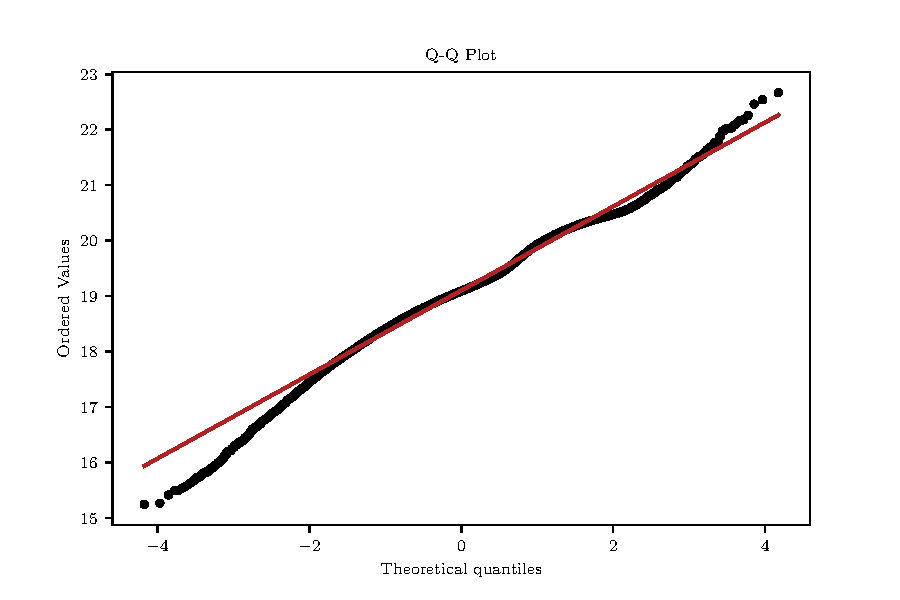
\includegraphics[width=\textwidth]{qq-plot}
	\caption{A Quantile-Quantile plot comparing theoretical quantiles of a normal distribution and the quantiles observed in the SDSS data.}
	\label{fig:qq}
\end{figure}
Observe in Figure~\ref{fig:qq} that towards the lower end of the theoretical quantiles there is significant deviation from the expected values; if the data were normally distributed, we would expect that the data points would fall on, or very near the red line. There is also slight evidence of departure from the expected quantiles towards the high-end of the plot.

\subsection*{Investigating Presence of Subpopulations}
Although our data \emph{looks} normally distributed on a histogram, every statistical test we've preformed has rejected the normality of the data. To understand why this is happening, we need to investigate what could be happening. We'll first plot the $r$ band magnitude using \emph{Scott's rule} for bin width. This will allow us to get a finer view of how our data is distributed than a normal histogram will.
\begin{figure}
	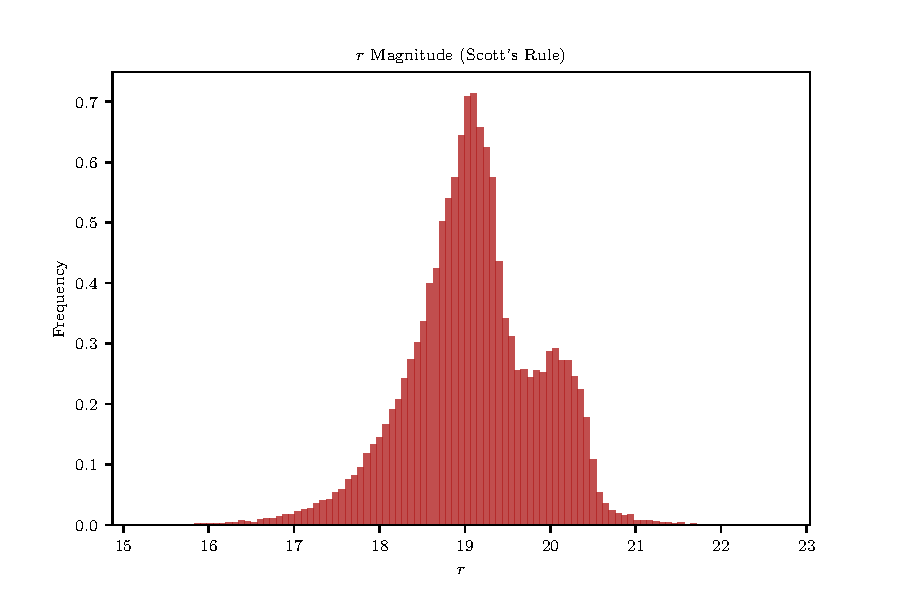
\includegraphics[width=\textwidth]{hist-scott}
	\caption{Histogram of $r$ band magnitudes, using \emph{Scott's rule} for determining bin width. Scott's rule says that the bin width $h$ should be equal to $\frac{3.5\hat{\sigma}}{n^{1/3}}$, where $\hat{\sigma}$ is the sample standard deviation and $n$ is the number of data points. In this example, $\hat{\sigma} \approx 0.76$ and $n = 46,420$.}
	\label{fig:hist-scott}
\end{figure}
Plotting the data using \emph{Scott's rule} shows us in Figure~\ref{fig:hist-scott} that our distribution appears to be bimodal, which did not show up at all on our original plot. We can investigate this apparent bimodality by looking at comparable histograms for the other passbands.
\begin{figure}
	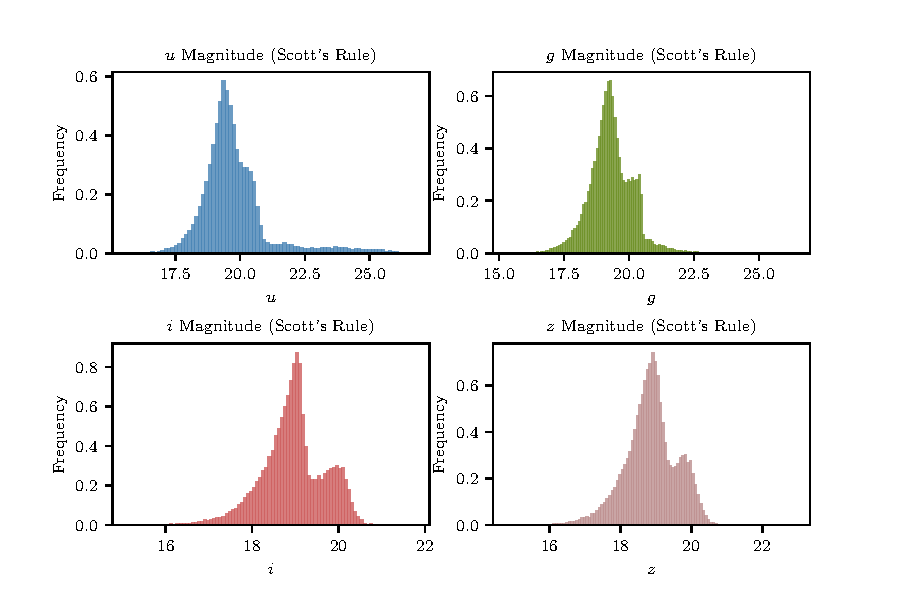
\includegraphics[width=\textwidth]{hist-colors}
	\caption{Passband magnitude histograms for the remaining color bands ($u,g,i,z$). Note the development of bimodality in the data as the color band gets progressively redder. }
	\label{fit:hist-colors}
\end{figure}

We discover that as our passbands get progressively more red, the bimodality of the brightness increases (Figure~\ref{fit:hist-colors}). When we look at brightness in the $u$ band, the data looks \emph{almost} normaly (still with significant evidence of non-normality), but in the $i$ and $z$ bands the presence of a second population of quasars is clearly visible on the histogram.
	\chapter{Conclusion}

Using data from the Sloan Digital Sky Survey, we analyzed photometric observations of some $46,000$ quasars. We first preformed principle component analysis on a subset of the features present in our dataset, finding that we could reduce our data to two primary components while retaining over $90\%$ of the inherent variation in the data. While this greatly improves the visualizability of the quasar observations, we lose a nice physical interpretation for what each component means. Next, we preformed regression on the $r - i$ color versus redshift ($z$) to attempt to find a predictor for color based on the redshift value of the quasar. We used residual analysis and the Bayesian/Akaike Information Criterions to determine what degree of polynomial best fit the data, as well as subset cross-validation to find that polynomials of degree $11$ or $12$ best model our data. We compare this to the graphs of fits found by \citeauthor{wu2003} in 2003. Finally, we preform hypothesis testing on the distribution of $r$ band magnitude observations, testing whether the brightness is likely drawn from a Gaussian parent distribution. Although an initial histogram plot of the observations made the data appear normal, the Anderson-Darling and Shapiro-Wilk tests indicated that there is sufficient evidence to reject the normality of the data, which is corroborated by examining a Quantile-Quantile plot of the data. By refining the bin width of the histogram using Scott's rule, we observed the presence of a distinct subpopulation of quasars with higher brightness measurements than the rest of the population. We then plotted histograms of the brightness measurements in all other colors bands and observe the trend that the subpopulation grows more distinct as the color band gets redder.

Areas for further investigation of this dataset are plentiful. My first idea is to look more closely at the presence of the subpopulations in band brightness observations, and attempt to identify the distinct parent distributions which combine to form the bimodal sample distribution observed in the data. I would also like to understand the physical interpretation for why these measurements are bimodal, and why increasing the redness of the passband differentiates between the two populations.
	\printbibliography
\end{document}
